% !TEX root = ../../report.tex
\section{Kinect}
\begin{Spacing}{\mylinespace}

\subsection{Aufbau und Funktion}

Die Kinect ist als eigenständige Bibliothek konzipiert und kann so in beliebige Projekte integriert werden. Das interne Vorgehen ist in Abbildung \ref{fig:kinectdll} schematisch dargestellt. 

\begin{figure}[hbtp]
	\vspace{0.2cm}
	\centering
	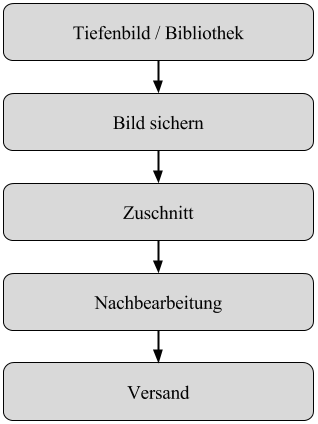
\includegraphics[width=0.6\textwidth]{graphics/block_dll.png}
	\caption{Laboraufbau}
	\label{fig:kinectdll}
\end{figure}

Nach dem Einbinden des Kinekt SDK kann sich ein Objekt der Kinect der Kinect erstellt sowie parametrisiert werden. Diese Objekt bietet nun die Möglichkeit sich auf einen Eventhandler zu registrieren, welcher die Auslieferung der Daten von Seitens der Kinect übernimmt. Dies wird alle in einem separaten Thread ausgeführt um die Leistung des Systems so optimal wie möglich zu halten.

Wird ein Bild empfangen wird, muss es als erstes in einer eigenen Struktur gesichert werden. Anschließend wird es auf die Zielauflösung zugeschnitten.
Dies ist nötig da der Sandkasten eine quadratische Form hat, das Bild jedoch im Format 3:4 (Auflösung von 640x480 Bildpunkte) von der Kinect kommt.
Als nächste Schritt muss der Bildaufbau verändert werden das das Bild um 180 Grad gedreht abgenommen wird. Dies hängt mit dem Hardwareaufbau zusammen, worin die Kinect befestigt ist. Weiterhin müssen die Tiefenwerte angepasst und auf die höhe des Sandkastens normiert werden. Der Grund hierfür liegt in der späteren Darstellung. Um die Farben der Höhenlinien angenehm verteilt anzeigen zu lassen, ist ein breites Spektrum an Tiefendaten erforderlich. Alle Bilddaten welche nicht im gewünschten Bereich des Sandkastens liegen werden auf unendlich gesetzt.

Abschließend werden die aufbereiteten Daten als Array mit einem Event verschickt und es kann ein weiteres Tiefenbild folgen. Für das Versenden wird deine eigene EventArgument-Klasse verwendet um eine spätere Erweiterung, z.B. hinzufügen von Metadaten, zu erleichtern.

\subsection{Nutzung}

Die Einbindung der Bibliothek ist über einen Verweis zu realisieren. Wenn die erfolgreich geschehen ist kann ein neues Objekt vom Typ "SandstormKinectCore" erstellt werden. Dieses Objekt bietet dann die Registrierung auf einen EventHandler an, welches genutzt werden soll.
Über die öffentlichen Methoden "StartKinect" sowie "StopKinect" kann nun der Betrieb hergestellt werden. Bei jedem neuen Tiefenbild wird über das Event ein Aufbereitetes Tiefenbild versand und kann weiter verwendet werden.

\end{Spacing}
\newpage
\clearpage
%% End Of Doc